\documentclass[10pt,a4paper]{article}

% ---------------------------------------------------------------- layout -----
\usepackage[a4paper,margin=2cm]{geometry}
\usepackage{fontspec}
\IfFontExistsTF{Arial}{\setmainfont{Arial}\setsansfont{Arial}}
                      {\setmainfont{Liberation Sans}\setsansfont{Liberation Sans}} % metric-compatible fallback
\renewcommand{\familydefault}{\sfdefault}
\usepackage{amsmath,amssymb}
\usepackage{graphicx}
\usepackage{booktabs}
\usepackage{float} % [H]: pin a figure exactly where it is written
\usepackage{tikz}
\usetikzlibrary{positioning,calc}
\usepackage{xcolor}
\usepackage[font=normalsize,labelfont=bf,skip=4pt]{caption}
\usepackage{enumitem}
\setlist{nosep,leftmargin=*}
\usepackage[numbers,sort&compress]{natbib}
\usepackage[hidelinks]{hyperref}
\usepackage{titlesec}
\titlespacing*{\section}{0pt}{8pt}{3pt}
\titlespacing*{\subsection}{0pt}{5pt}{2pt}
\titleformat*{\section}{\large\bfseries}
\titleformat*{\subsection}{\normalsize\bfseries}
\setlength{\parskip}{3pt}
\setlength{\parindent}{0pt}
\setlength{\textfloatsep}{8pt}
\setlength{\floatsep}{6pt}
\setlength{\emergencystretch}{3em}

% Placeholders the team must fill in are shown in red.
\newcommand{\TODO}[1]{\textcolor{red}{[#1]}}
\newcommand{\bpb}{\text{BPB}}
\newcommand{\dd}{\Delta}

\begin{document}
% Front matter reuses page 1; reserve hyperlink page anchors for the main text.
\hypersetup{pageanchor=false}

% =============================================================== COVER =======
\begin{titlepage}
\centering
\vspace*{2.5cm}
{\large SC4001 Neural Networks and Deep Learning --- Group Project\par}
\vspace{1.5cm}
{\LARGE\bfseries Growing the Vocabulary Without Growing the Embedding:\\[4pt]
Compact Tied Embeddings for Vocabulary Scaling\\[4pt] under Fixed Storage and Compute\par}
\vspace{1.8cm}
{\large Group 189 \par}
\vspace{0.8cm}
\begin{tabular}{ll}
Tan Xeng Ian & \TODO{Matriculation no.}\\
Low King Whey & U2423402K\\
\TODO{Josh Lai} & \TODO{Matriculation no.}\\
\end{tabular}
\vfill
{Code and frozen results: \url{https://github.com/tanXeng/SC4001_compact_embeddings}\\
branch \texttt{research/vocab-scaling-fp32-isoflops}\par}
\vspace{0.6cm}
{Nanyang Technological University, November 2026\par}
\end{titlepage}

% ============================================================ CONTENTS =======
\tableofcontents
\clearpage
\setcounter{page}{1}
\hypersetup{pageanchor=true}

% ============================================================ ABSTRACT =======
\begin{center}
{\large\bfseries Abstract}
\end{center}
\vspace{-4pt}
\noindent
Larger subword vocabularies compress text into fewer tokens, but in a small language model the
$V\times d$ embedding table, and the tied output softmax that reuses it, grow linearly with the vocabulary
size $V$. We ask whether \emph{compact} embedding representations let a model use a larger vocabulary
without paying for it, when both the vocabulary's storage and the training compute are held fixed. We
train a pre-LayerNorm Transformer with 32M non-embedding parameters on FineWeb with nested byte-level BPE vocabularies of
16K, 32K and 64K types. Every arm receives exactly $5\times10^{17}$ estimated training FLOPs, and every
compact arm must fit its serialised vocabulary into the bytes of the dense 16K table (33.6\,MB). We
compare a dense baseline, low-rank factorisation (ALBERT-style), adaptive input representations and hash
embeddings, all adapted to an exactly tied full softmax, plus uncapped dense 32K/64K controls. Quality is
measured in tokenizer-independent bits per byte (\bpb) on a screening split and on a document-disjoint
confirmation split that was evaluated only once. At equal storage and compute, Adaptive 64K obtains the
best confirmation \bpb{} of all eight arms (1.2689 vs.\ 1.2880 for the 16K baseline), beating even
the dense 64K control that uses $4\times$ the storage. Low-rank 32K recovers 94\% of the dense 32K
gain at half its storage. Hash 64K is clearly worse than the baseline (1.3789). We show analytically and
empirically that factorised tied embeddings also shrink the output-softmax cost, which converts saved
bytes into roughly 50\% more optimiser updates than dense 64K. Hash collisions fall hardest on rare
tokens, which lose up to 3.5 nats relative to dense 64K. These results come from a single seed
and a single budget; we report them as such.

% ======================================================== INTRODUCTION =======
\section{Introduction}
\label{sec:intro}

The vocabulary is a hidden scaling axis of language models. A larger subword vocabulary makes each
token cover more text: in our data, a 16K BPE vocabulary averages 4.14 raw bytes per token, while 64K
averages 4.60 (+11\%). For a fixed backbone, this means more text is processed per FLOP and the model
predicts more text per position of context. The price is paid in the vocabulary layer. A dense table
$E\in\mathbb{R}^{V\times d}$ costs $Vd$ parameters. With weight tying \citep{press2017tying,inan2017tying},
the same table also forms the output projection, which costs $2Vd$ FLOPs per token in the forward pass.
Throughout, a \emph{small} model is one whose backbone has fewer than 50M parameters, the ceiling our
framework enforces; ours has 32.0M (10 layers, $d=512$). At this scale the vocabulary is a large share of
the model. A dense 16K table already holds 8.4M parameters (33.6\,MB in FP32), 21\% of all parameters. A
dense 64K table holds 33.6M (134\,MB), \emph{more than the whole backbone}, so over half of the dense 64K
model is vocabulary. Its output layer costs 67M FLOPs per token, about 80\% of the entire backbone's 84M. Recent work on vocabulary scaling laws
\citep{tao2024vocab} finds that the compute-optimal vocabulary grows with model size. This suggests that
small models cannot afford large vocabularies.

\emph{Compact embeddings} (low-rank factorisation \citep{lan2020albert}, hash embeddings
\citep{svenstrup2017hash} and adaptive, frequency-banded representations \citep{baevski2019adaptive}) all
cut the parameter cost of the vocabulary. They are usually judged on memory saved for a fixed
vocabulary. We turn the question around and ask whether these methods can \emph{relocate the optimum}:
can a small model use a larger vocabulary if the vocabulary is stored compactly? Answering this fairly
requires two budgets at once. With storage alone fixed, a compact arm could train for longer. With compute
alone fixed, a dense arm could keep more parameters. We therefore study:
\begin{itemize}
  \item \textbf{RQ1.} With the vocabulary's serialised storage capped at the dense 16K table and the
  training FLOPs fixed, does a compact 32K or 64K vocabulary beat the dense 16K baseline?
  \item \textbf{RQ2.} How much of the gain of an \emph{uncapped} dense 32K/64K model does each compact
  representation recover, and why?
  \item \textbf{RQ3.} Which tokens pay for compression, and what do the learned representations reveal
  about each method's failure modes?
\end{itemize}

\textbf{Contributions.} (i) A dual-budget protocol: a byte-exact storage cap on the actual serialised
vocabulary archive, together with iso-FLOP training of complete optimiser updates. Evaluation uses
tokenizer-independent \bpb{} and a once-only, document-disjoint confirmation split. (ii) Adaptations of
low-rank, adaptive and hash embeddings to an \emph{exactly tied, full-softmax} causal LM over BPE subwords.
(iii) The finding that the best compact arm (Adaptive 64K) beats every dense arm, using approximately the same
storage as Dense 16K, half that of Dense 32K and a quarter that of Dense 64K. We give an analysis showing that \emph{factorised} tied embeddings (Low-rank and Adaptive, which
store a small table times a projection instead of the full $V\times d$ table) cap the softmax cost at twice
the vocabulary parameter count, which turns saved bytes into extra optimiser updates. (iv) Frequency-group and
representation diagnostics (spectra, band conditioning, hash occupancy and gradient interference) that
explain the ranking, including a controlled negative result for hash embeddings.

% ============================================================ RELATED ========
\section{Review of Existing Techniques}
\label{sec:related}

\textbf{Vocabulary size and its cost.} Subword tokenisers such as BPE \citep{sennrich2016bpe} and its
byte-level variant \citep{radford2019gpt2} trade vocabulary size against sequence length. Scaling-law
studies \citep{kaplan2020scaling,hoffmann2022chinchilla} usually exclude embedding parameters, but
\citet{tao2024vocab} show that the vocabulary matters for compute-optimal training and that the optimal
$V$ grows with non-embedding parameters. Weight tying
\citep{press2017tying,inan2017tying} shares the input and output matrices. This halves the parameters but
leaves the output softmax, whose cost is $O(Vd)$ per token. For a small model, the softmax is often the
single largest matrix multiply.

\textbf{Low-rank factorisation.} ALBERT \citep{lan2020albert} factorises the embedding as
$E=AB$ with $A\in\mathbb{R}^{V\times r}$ and $B\in\mathbb{R}^{r\times d}$, reducing parameters from $Vd$ to
$r(V+d)$. The motivation is that context-independent token embeddings need less capacity than hidden
states. ALBERT applies this on the input side of a masked encoder. In a tied LM, the factorisation also
constrains the logit matrix to rank $\le r$, the \emph{softmax bottleneck} identified by
\citet{yang2018softmax}. Whether this harms a causal LM at small $r$ is therefore an open empirical question.

\textbf{Hash embeddings.} Feature hashing \citep{weinberger2009hashing} maps tokens to a fixed number of
buckets, so that colliding tokens share an identical vector. \citet{svenstrup2017hash} reduce the
damage of collisions. Each token selects $k$ component vectors from a shared pool of $B$ vectors using $k$
hash functions and combines them with $k$ trainable \emph{importance} weights. Two tokens then coincide
only if all $k$ indices collide, and the weights let the model separate partial collisions. The method was
evaluated on text classification, where the embeddings are only read on the input side.

\textbf{Adaptive representations.} The adaptive softmax \citep{grave2017adaptivesoftmax} partitions the
vocabulary by frequency and gives rare clusters smaller capacity in a hierarchical output layer. Adaptive
input representations \citep{baevski2019adaptive} carry the idea to the input: band $j$ has dimension
$d/k^{j}$ (typically $k=4$) and is linearly projected to $d$. Tying the bands with an adaptive softmax gave
faster training and lower perplexity on word-level WikiText-103. This allocation follows the Zipfian
prior that frequent tokens deserve more capacity.

\textbf{Other approaches and gap.} Compositional codes \citep{shu2018compositional} and tensor-train
embeddings \citep{hrinchuk2020tensorized} compress the table further, at the cost of more complex
decoding. Rare-token embeddings are known to degenerate in tied generative models \citep{gao2019degeneration},
so compression may hurt the tail most. Previous studies compare these methods (i) at a \emph{fixed
vocabulary}, (ii) on parameter counts rather than actual bytes, (iii) mostly on input-side or word-level
tasks, and (iv) rarely with matched training compute. None asks whether compact storage lets a small
subword LM afford a larger vocabulary under both budgets. That is the question we address.

% ============================================================ METHODS ========
\section{Methods}
\label{sec:methods}

\subsection{Model and tied vocabulary interface}
All arms share one backbone: a 10-layer pre-LayerNorm \citep{xiong2020preln} causal Transformer
\citep{vaswani2017attention} with width $d=512$, 8 heads, FFN width 2048, learned positions (context
1024), GELU and dropout 0.1. It has 32,033,792 non-vocabulary parameters. A vocabulary module exposes two
operations that share \emph{the same} parameters: \texttt{lookup}$(w)\in\mathbb{R}^{d}$ returns the input
row $e_w$, and \texttt{project}$(h)=hE^{\top}\in\mathbb{R}^{V}$ returns the logits of a \emph{full,
exact} softmax over the effective table $E$. Only the vocabulary module differs between arms. All weights
are FP32, so storage is never traded for precision.

\subsection{Vocabulary representations}
\label{sec:reps}

\textbf{Dense} (baseline and controls): $E$ is a free $V\times d$ matrix.

\textbf{Low-rank} \citep{lan2020albert}: $e_w = a_w B$, with $A\in\mathbb{R}^{V\times r}$ and
$B\in\mathbb{R}^{r\times d}$. Logits are computed as $(hB^{\top})A^{\top}$, so $E$ is never materialised.

\textbf{Adaptive} \citep{baevski2019adaptive}: token types are sorted by \emph{training-set} frequency
(EOS forced into the head) and split into three bands of sizes $n_1,n_2,n_3$ with widths
$d_j=512/4^{\,j-1}=512,128,32$. Band $j$ owns a table $A_j\in\mathbb{R}^{n_j\times d_j}$ and a
projection $B_j\in\mathbb{R}^{d_j\times d}$, and $e_w=a_{w}B_{j(w)}$. \emph{Adaptation:} instead of the
hierarchical adaptive softmax, the output computes all band logits $(hB_j^{\top})A_j^{\top}$ and
concatenates them into one exact full softmax. The input and output are therefore exactly tied, and the
loss is directly comparable with the other arms.

\textbf{Hash} \citep{svenstrup2017hash}: a shared pool $C\in\mathbb{R}^{B\times d}$ and $k=2$
deterministic hash functions $h_i(w)=\mathrm{SHA256}(\text{seed}_i, w) \bmod B$ (seeds 17, 29). Each token
has learned importance weights $p_w\in\mathbb{R}^{2}$, initialised $\mathcal{N}(0,1/k)$, and
$e_w = \sum_{i=1}^{2} p_{w,i}\, c_{h_i(w)}$. \emph{Adaptations:} the BPE vocabulary is closed, so
importance weights are stored per token instead of via a second hash. The effective table is materialised
once per forward pass and tied to the output softmax. The paper used hash embeddings only on the input
side; tying them to the output is, to our knowledge, untested.

\begin{figure}[H] 
\centering
\resizebox{\linewidth}{!}{%
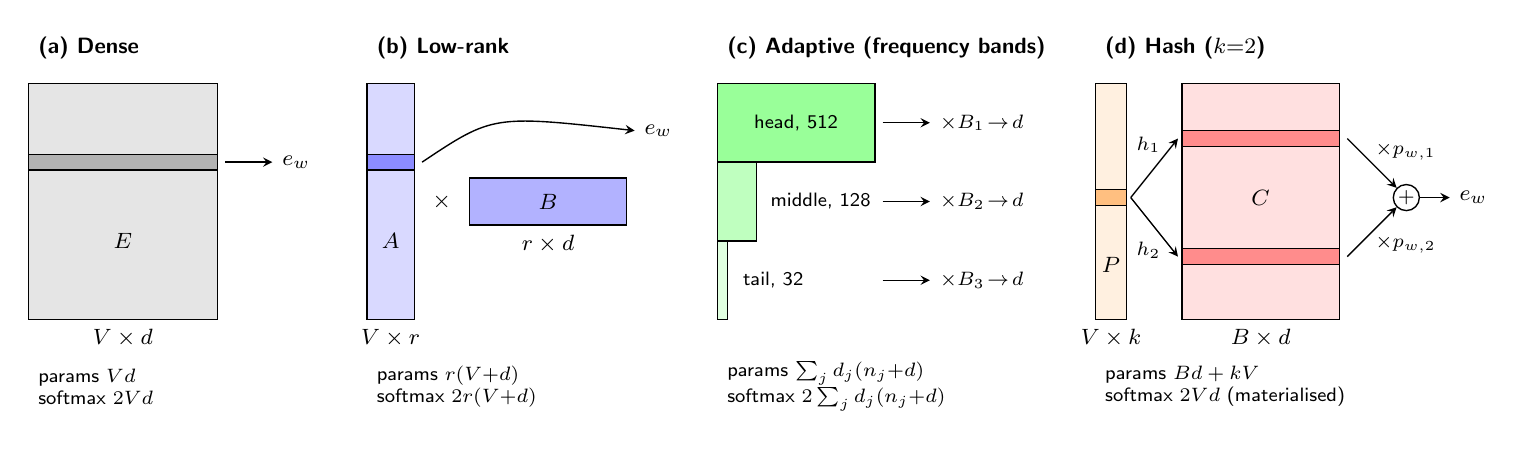
\begin{tikzpicture}[font=\footnotesize, >=stealth, line width=.5pt]
  % ---------------- (a) Dense
  \node[anchor=west,font=\footnotesize\bfseries] at (0,3.45) {(a) Dense};
  \draw[fill=gray!20] (0,0) rectangle (2.4,3.0);
  \draw[fill=gray!60] (0,1.9) rectangle (2.4,2.1);
  \node at (1.2,1.0) {$E$};
  \node[below] at (1.2,0) {$V\times d$};
  \draw[->] (2.5,2.0) -- (3.1,2.0) node[right] {$e_w$};
  \node[anchor=west,align=left,font=\scriptsize] at (0,-0.85) {params $Vd$\\softmax $2Vd$};
  % ---------------- (b) Low-rank
  \begin{scope}[xshift=4.3cm]
  \node[anchor=west,font=\footnotesize\bfseries] at (0,3.45) {(b) Low-rank};
  \draw[fill=blue!15] (0,0) rectangle (0.6,3.0);
  \draw[fill=blue!45] (0,1.9) rectangle (0.6,2.1);
  \node at (0.3,1.0) {$A$};
  \node[below] at (0.3,0) {$V\times r$};
  \node at (0.95,1.5) {$\times$};
  \draw[fill=blue!30] (1.3,1.2) rectangle (3.3,1.8);
  \node at (2.3,1.5) {$B$};
  \node[below] at (2.3,1.2) {$r\times d$};
  \draw[->] (0.7,2.0) .. controls (1.6,2.6) .. (3.4,2.4) node[right] {$e_w$};
  \node[anchor=west,align=left,font=\scriptsize] at (0,-0.85) {params $r(V{+}d)$\\softmax $2r(V{+}d)$};
  \end{scope}
  % ---------------- (c) Adaptive
  \begin{scope}[xshift=8.75cm]
  \node[anchor=west,font=\footnotesize\bfseries] at (0,3.45) {(c) Adaptive (frequency bands)};
  \draw[fill=green!40] (0,2.0) rectangle (2.0,3.0);
  \draw[fill=green!25] (0,1.0) rectangle (0.5,2.0);
  \draw[fill=green!12] (0,0) rectangle (0.125,1.0);
  \node[font=\scriptsize] at (1.0,2.5) {head, 512};
  \node[font=\scriptsize,anchor=west] at (0.55,1.5) {middle, 128};
  \node[font=\scriptsize,anchor=west] at (0.2,0.5) {tail, 32};
  \draw[->] (2.1,2.5) -- (2.7,2.5) node[right,font=\scriptsize] {$\times B_1\!\to\! d$};
  \draw[->] (2.1,1.5) -- (2.7,1.5) node[right,font=\scriptsize] {$\times B_2\!\to\! d$};
  \draw[->] (2.1,0.5) -- (2.7,0.5) node[right,font=\scriptsize] {$\times B_3\!\to\! d$};
  \node[anchor=west,align=left,font=\scriptsize] at (0,-0.85) {params $\sum_j d_j(n_j{+}d)$\\softmax $2\sum_j d_j(n_j{+}d)$};
  \end{scope}
  % ---------------- (d) Hash
  \begin{scope}[xshift=13.55cm]
  \node[anchor=west,font=\footnotesize\bfseries] at (0,3.45) {(d) Hash ($k{=}2$)};
  % per-token weights P (V x k), row w highlighted
  \draw[fill=orange!12] (0,0) rectangle (0.4,3.0);
  \draw[fill=orange!50] (0,1.45) rectangle (0.4,1.65);
  \node at (0.2,0.7) {$P$};
  \node[below] at (0.2,0) {$V\times k$};
  % shared pool C (B x d), the two rows selected by h_1(w), h_2(w)
  \draw[fill=red!12] (1.1,0) rectangle (3.1,3.0);
  \draw[fill=red!45] (1.1,2.2) rectangle (3.1,2.4);
  \draw[fill=red!45] (1.1,0.7) rectangle (3.1,0.9);
  \node at (2.1,1.55) {$C$};
  \node[below] at (2.1,0) {$B\times d$};
  \draw[->] (0.45,1.55) -- node[pos=0.7,above left,font=\scriptsize,inner sep=1pt] {$h_1$} (1.05,2.3);
  \draw[->] (0.45,1.55) -- node[pos=0.7,below left,font=\scriptsize,inner sep=1pt] {$h_2$} (1.05,0.8);
  % weighted sum -> e_w
  \node[draw,circle,inner sep=0.5pt,font=\scriptsize] (sum) at (3.95,1.55) {$+$};
  \draw[->] (3.2,2.3) -- node[above right,font=\scriptsize,inner sep=1pt] {$\times p_{w,1}$} (sum);
  \draw[->] (3.2,0.8) -- node[below right,font=\scriptsize,inner sep=1pt] {$\times p_{w,2}$} (sum);
  \draw[->] (sum) -- (4.5,1.55) node[right] {$e_w$};
  \node[anchor=west,align=left,font=\scriptsize] at (0,-0.85) {params $Bd + kV$\\softmax $2Vd$ (materialised)};
  \end{scope}
\end{tikzpicture}}
\caption{The four tied vocabulary representations. Each produces the input row $e_w$ and, through the
same parameters, the output logits $hE^{\top}$ of a full softmax. The bottom lines give the parameter
count and the forward softmax FLOPs per token (Sec.~\ref{sec:flops}).}
\label{fig:schematic}
\end{figure}

\subsection{Budget 1: a byte-exact storage cap}
\label{sec:storage}
The cap is the size of the \emph{actual} \texttt{torch.save} archive of the dense 16K table,
33,555,740 bytes, including container overhead. Each compact arm counts every persistent tensor in its
archive: parameters, hash index buffers and the adaptive permutation. Each compact arm is given the largest
configuration that fits. A binary search verifies that the chosen size fits and that the next size up does
not. The allocation rule never sees validation data:
\begin{itemize}
  \item Low-rank: $r=252$ (32K) and $r=127$ (64K), 99.98\% and 99.99\% of the cap.
  \item Adaptive: the middle band is fixed at $V/4$, and the head is the largest multiple of 256 that fits.
        Cutoffs are $[12544, 20736]$ (32K) and $[8448, 24832]$ (64K), 99.3\% of the cap.
  \item Hash (64K only, the most severe $4\times$ compression): $B=15{,}615$ components, 99.996\% of the cap.
\end{itemize}
Full table shapes, parameter counts and archive bytes for every arm are in Table~\ref{tab:config} (Appendix~\ref{app:details}).
Dense 32K and 64K use $2\times$ and $4\times$ the cap. They are \emph{exempt controls} that show what an
uncompressed larger vocabulary achieves.

\subsection{Budget 2: iso-FLOP training, and why representation changes compute}
\label{sec:flops}
Each arm trains until it has spent $5\times10^{17}$ estimated FLOPs: training stops when the next
complete optimiser update would exceed the budget, leaving less than 0.002\% unused. The estimator counts
forward and backward matrix multiplications (GEMMs), full causal attention and executed padding, including each representation's own
graph (for Adaptive, an upper bound on the input side). It excludes the optimiser, loss, normalisation and
indexing. This is a fixed accounting convention, not measured hardware work.

The vocabulary choice changes how many updates fit in this budget. The forward cost of the tied
output layer per token is
\begin{equation}
C_{\text{out}} = \underbrace{2Vd}_{\text{dense, hash}},\qquad
\underbrace{2r(V+d)}_{\text{low-rank}},\qquad
\underbrace{2\textstyle\sum_j d_j(n_j+d)}_{\text{adaptive}} .
\label{eq:cout}
\end{equation}
For both factorised representations, $C_{\text{out}}$ equals exactly \emph{twice the vocabulary
parameter count}, so a storage cap is also a cap on softmax compute. Our implemented Hash output path
materialises the table and therefore still costs $2Vd$ for the output projection. For $V{=}65{,}536$, $d{=}512$,
Eq.~\eqref{eq:cout} gives 67.1M FLOPs per token for dense or hash, against 16.8M for low-rank and 16.1M for
adaptive. The backbone costs $\approx$84M FLOPs per token (63M in its weight matrices and 21M in
full-square attention). The measured cost per update (Table~\ref{tab:main}) is
$14.6\times10^{12}$ FLOPs for Dense/Hash 64K and $9.8\times10^{12}$ for all factorised arms and the 16K
baseline. Under iso-FLOPs, a dense 64K model therefore gets one third fewer updates.

% =========================================================== SETUP ===========
\section{Experimental Setup}
\label{sec:setup}

\textbf{Data.} FineWeb \citep{penedo2024fineweb} \texttt{sample-10BT} at a pinned revision. Two parquet
shards are deterministically split by document (seed 42) after global exact-text deduplication. The
result is a training pool of 1,137,468 documents (3.50\,GB) and 3,219 validation documents (10.0\,MB),
which are disjoint. Training windows never attend across document boundaries.

\textbf{Tokenisers.} One byte-level BPE family is fitted only on the first 65,182 training documents
(200\,MB). It has no normalisation, and EOS has ID 0. The vocabularies are nested: the 64K merge list
extends the 32K list exactly. The 32K and 64K arms therefore differ only in what they add, which isolates the
effect of vocabulary size.

\textbf{Training.} AdamW \citep{loshchilov2019adamw} (lr $3{\times}10^{-4}$, $\beta=(0.9,0.999)$, weight
decay 0.01, constant schedule) with gradient clipping at 1.0. Each update uses 32 windows of 1024 tokens
(microbatch 16 $\times$ 2 accumulation steps, stride 512). Training uses seed 42 and FP32 with TF32
disabled, and every arm sees the same deterministic data order. Each arm ran on one NVIDIA A40 with
atomic checkpoints every 300\,s and exact resume. No hyperparameter was tuned per arm: settings are fixed
in versioned YAML protocols, and ranks, cutoffs and pool sizes were chosen by a storage-fitting rule that
never uses validation quality. We ran 8 arms (Table~\ref{tab:main}).

\textbf{Evaluation.} Token-level loss is not comparable across tokenisers, so we report \emph{bits per
byte} \citep{gao2020pile}: $\bpb=\sum_t \mathrm{NLL}_t / (\ln 2\cdot\#\text{raw UTF-8 bytes})$, where
$\mathrm{NLL}_t=-\ln p(x_t\mid x_{<t})$ is the negative log-likelihood of target token $t$. NLL is
measured in \emph{nats}, the natural-log unit of information ($1\text{ nat}=1/\ln 2\approx1.44$ bits),
so the factor $\ln 2$ converts the total to bits. Every document is scored with windows of length 1024
and stride 512. Each target, including EOS, is scored exactly
once. We use two document-disjoint validation subsets of 256 documents each. \emph{Screening} (750\,KB)
was evaluated at 0, 25, 50, 75 and 100\% of the budget for learning curves. \emph{Confirmation} (677\,KB)
was evaluated \emph{once} per arm, at the end of training. For diagnosis, we split token types into equal-count
\emph{thirds} by training frequency rank (or by band, for Adaptive) and report the NLL for each group. At
50\% and 100\% of the budget we also record spectra of the effective embeddings, band conditioning, hash
occupancy and collisions, and a bounded gradient-interference probe for shared hash components.

% ========================================================== RESULTS ==========
\section{Results}
\label{sec:results}

\begin{table}[H]
\centering
\caption{Main results. All arms use $5\times10^{17}$ training FLOPs. Storage is the serialised
vocabulary archive, as a multiple of the 16K dense cap (33.56\,MB). Text is the raw UTF-8 training text
consumed within the budget. $\dd$ is the change in confirmation
\bpb{} relative to the baseline; lower is better. GPU-h is active training time on one A40; Mem is the
peak allocated training memory. Parameter counts are in Table~\ref{tab:config} (Appendix~\ref{app:details}). * marks controls that exceed the storage cap. Best capped arm in bold.}
\label{tab:main}
\setlength{\tabcolsep}{3.5pt}
\begin{tabular}{@{}llrrrrrrrr@{}}
\toprule
Arm & Rep. hyper-params & Storage & Updates & Text & Screen & Confirm & $\dd$ conf. & GPU-h & Mem \\
 & & ($\times$cap) & & (GB) & \bpb & \bpb & & & (GiB)\\
\midrule
Dense 16K (base) & --- & 1.00 & 50,962 & 2.54 & 1.2723 & 1.2880 & --- & 10.0 & 9.9\\
\midrule
Dense 32K* & --- & 2.00 & 43,848 & 2.28 & 1.2564 & 1.2729 & $-$0.0151 & 9.8 & 14.0\\
Low-rank 32K & $r=252$ & 1.00 & 51,027 & 2.66 & 1.2600 & 1.2738 & $-$0.0142 & 10.4 & 13.9\\
Adaptive 32K & 512/128/32 & 0.99 & 51,081 & 2.66 & 1.2654 & 1.2778 & $-$0.0102 & 17.5 & 13.9\\
\midrule
Dense 64K* & --- & 4.00 & 34,207 & 1.83 & 1.2574 & 1.2744 & $-$0.0136 & 9.7 & 22.2\\
Low-rank 64K & $r=127$ & 1.00 & 51,243 & 2.74 & 1.2632 & 1.2782 & $-$0.0098 & 11.4 & 21.9\\
Adaptive 64K & 512/128/32 & 0.99 & 51,368 & 2.75 & \textbf{1.2545} & \textbf{1.2689} & $\mathbf{-0.0191}$ & 25.7 & 21.9\\
Hash 64K & $B{=}15615,k{=}2$ & 1.00 & 34,205 & 1.83 & 1.3585 & 1.3789 & $+$0.0909 & 9.7 & 22.3\\
\bottomrule
\end{tabular}
\end{table}

\subsection{Main comparison (RQ1, RQ2)}
Table~\ref{tab:main} and Fig.~\ref{fig:tradeoff}a summarise the eight arms.\\
\textbf{RQ1: yes, for factorised representations.} All four factorised compact arms beat the 16K baseline
on both splits while using no more vocabulary storage than it does. The confirmation gains range from
$-0.0098$ (Low-rank 64K) to $-0.0191$ \bpb{} (Adaptive 64K, $-1.5\%$ relative). Hash 64K is the
exception: it is \emph{worse} than the baseline by $+0.091$ \bpb.

\textbf{RQ2: recovery of the dense gain.} Recovery
$=(\bpb_{\text{base}}-\bpb_{\text{arm}})/(\bpb_{\text{base}}-\bpb_{\text{dense}})$, where the dense control
has the same vocabulary size; values above 100\% mean the arm beats that control. At 32K, Low-rank recovers 94\% of the Dense 32K confirmation gain
(77\% on screening) at half the storage; Adaptive recovers 67\% (43\%). At 64K the picture inverts.
Low-rank recovers 72\% (61\%), while Adaptive \emph{exceeds} the uncapped Dense 64K control, reaching
140\% (119\%) of its gain at a quarter of the storage. Adaptive 64K is the best arm overall on both splits,
including both dense controls. Dense scaling alone does not pay off at this budget: Dense 64K is slightly
worse than Dense 32K on both splits (1.2744 vs.\ 1.2729 confirmation). This is consistent with the
argument of \citet{tao2024vocab} that a small model cannot afford a very large vocabulary. With compact
storage, however, the 64K vocabulary becomes the best choice. The ranking is stable between screening and
confirmation, except that Dense 64K and Low-rank 32K swap places, and they differ by only 0.0006--0.0026.
With a single seed, we treat differences of a few thousandths as unresolved.

\begin{figure}[H]
\centering
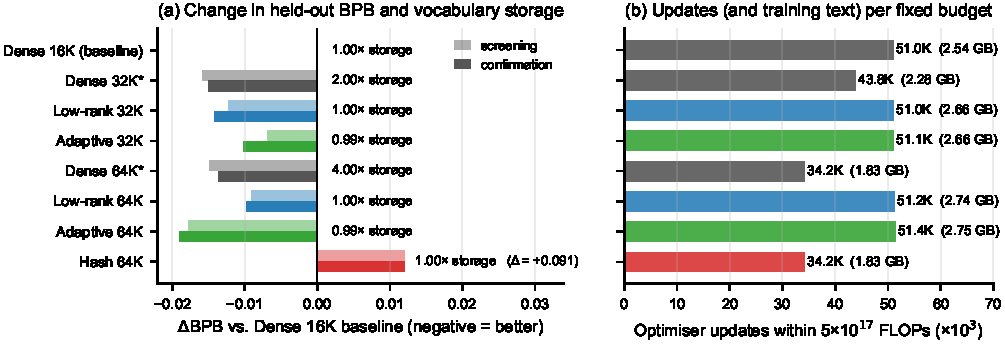
\includegraphics[width=\linewidth]{figures/fig_tradeoff.pdf}
\caption{(a) Change in held-out \bpb{} relative to the Dense 16K baseline (pale: screening, dark:
confirmation), annotated with each arm's vocabulary storage relative to the cap. Hash is clipped; its value
is printed. (b) Optimiser updates and training text processed within the same $5\times10^{17}$ FLOPs.
Dense and Hash 64K pay for a $2Vd$ softmax and receive one third fewer updates.}
\label{fig:tradeoff}
\end{figure}

\subsection{Where the gains come from: compute reallocation}
Figure~\ref{fig:tradeoff}b confirms the analysis of Sec.~\ref{sec:flops}. Every factorised arm
completes about 51K updates, the same number as the 16K baseline, because Eq.~\eqref{eq:cout} keeps their
softmax at baseline cost. Dense 32K completes 14\% fewer updates, and Dense 64K and Hash 64K complete 33\%
fewer. The larger vocabulary also compresses text better (4.41 and 4.60 bytes per token at 32K and 64K, against 4.14
at 16K). The factorised 64K arms therefore read 2.75\,GB of text against 2.54\,GB for the baseline and
1.83\,GB for Dense 64K. The benefit of a compact vocabulary is thus twofold. It removes the storage cost,
and, more importantly under iso-FLOPs, it removes the softmax cost that would otherwise erase the
compression gain of a large vocabulary.

Hash 64K and Dense 64K provide a clean control. They completed the same number of updates (34,205 vs.\
34,207) on the same data stream at the same FLOPs. Their entire 0.105 \bpb{} gap (confirmation) is
therefore caused by the representation, and Hash 64K pays the dense compute cost without the dense
capacity. Conversely, Low-rank 64K receives 50\% more updates than Dense 64K yet still loses by 0.004--0.006
\bpb. For a rank of $r=127$, the capacity cost outweighs the extra data at this budget.

\begin{figure}[H]
\centering
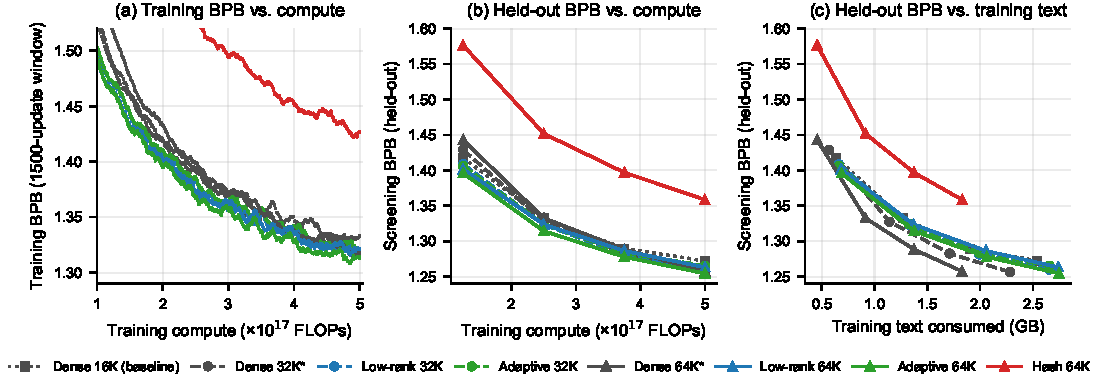
\includegraphics[width=\linewidth]{figures/fig_curves.pdf}
\caption{Learning curves. (a) Training \bpb{}, as the exact ratio of summed NLL to summed bytes over a
1,500-update moving window (shown from 20\% of the budget). (b) Held-out screening \bpb{} at 25/50/75/100\%
of the FLOP budget (exact values in Table~\ref{tab:budget}, Appendix~\ref{app:details}). (c) The same held-out points plotted against the training text consumed (sample
efficiency). Colour shows the representation, and line style shows the vocabulary size (dotted 16K,
dashed 32K, solid 64K).}
\label{fig:curves}
\end{figure}

\subsection{Learning dynamics}
Figure~\ref{fig:curves} shows that the advantage of factorised arms is largest early and narrows with
compute. At 25\% of the budget, Low-rank 64K and Adaptive 64K lead Dense 64K by 0.042 and 0.047 screening
\bpb{}, and the factorised 32K arms lead Dense 32K by about 0.02. By the end, both dense controls have
overtaken their low-rank counterparts. The crossover falls between 75\% and 100\% (at 75\%,
Low-rank 64K still leads, 1.2862 vs.\ 1.2884). Adaptive 64K is the only arm that stays ahead of its dense
control throughout. The training \bpb{} over the final 2,000 updates is
Adaptive 64K 1.312, Dense 32K 1.315, Low-rank 32K 1.315, Dense 64K 1.319, Low-rank 64K 1.319,
Adaptive 32K 1.320, baseline 1.333, Hash 1.428. Every arm sees each document at most once, so there is no
sign of differential overfitting.

Figure~\ref{fig:curves}c separates \emph{sample} efficiency from \emph{compute} efficiency. At equal
training text ($\approx$1.37\,GB, which is also $\approx$25.6K updates for every 64K arm), Dense 64K
reaches 1.288 \bpb{}, against 1.314 for Adaptive 64K and 1.324 for Low-rank 64K. Per update, the full
dense table is clearly the better learner. The compact arms win at the end only because each of their
updates costs about a third less (Eq.~\eqref{eq:cout}). The crossovers indicate that the \emph{size} of the compact advantage depends
on the budget. Low-rank's lead comes from extra updates, and that lead shrinks as training proceeds.

\begin{figure}[H]
\centering
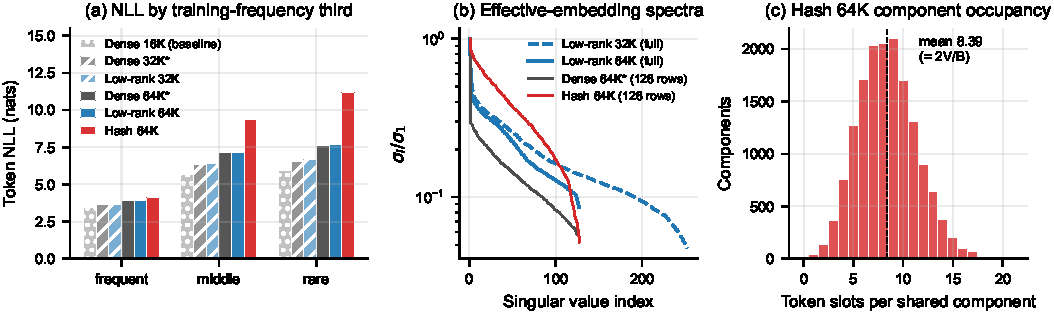
\includegraphics[width=\linewidth]{figures/fig_frequency_diagnostics.pdf}
\caption{(a) Confirmation NLL by training-frequency third of token types (thirds are defined within each
vocabulary, so compare bars of the same size). (b) Normalised singular spectra: the full effective
spectrum for low-rank, and 128 evenly spaced token rows for dense and hash. (c) Hash 64K: the number of
token slots that share each of the 15,615 components.}
\label{fig:freq}
\end{figure}

\begin{table}[H]
\centering
\caption{Confirmation token NLL (nats) and accuracy by training-frequency third of token types. Mass is
each group's share of confirmation targets. Thirds are defined within each vocabulary, so compare rows only
within a vocabulary size. Adaptive is omitted because its natural groups are its bands, not thirds.}
\label{tab:freq}
\begin{tabular}{@{}lrrrrrrrrr@{}}
\toprule
 & \multicolumn{3}{c}{Frequent third} & \multicolumn{3}{c}{Middle third} & \multicolumn{3}{c}{Rare third}\\
\cmidrule(lr){2-4}\cmidrule(lr){5-7}\cmidrule(lr){8-10}
Arm & NLL & Acc. & Mass & NLL & Acc. & Mass & NLL & Acc. & Mass\\
\midrule
Dense 16K    & 3.431 & .360 & .876 & 5.685 & .223 & .086 & 5.904 & .222 & .039\\
\midrule
Dense 32K*   & 3.679 & .337 & .910 & 6.364 & .192 & .064 & 6.554 & .206 & .027\\
Low-rank 32K & 3.675 & .339 & .910 & 6.417 & .190 & .064 & 6.656 & .197 & .027\\
\midrule
Dense 64K*   & 3.896 & .319 & .942 & 7.160 & .182 & .043 & 7.623 & .165 & .016\\
Low-rank 64K & 3.909 & .325 & .942 & 7.158 & .180 & .043 & 7.666 & .169 & .016\\
Hash 64K     & 4.095 & .310 & .942 & 9.338 & .111 & .043 & 11.164 & .052 & .016\\
\bottomrule
\end{tabular}
\end{table}

\subsection{Which tokens pay for compression? (RQ3)}
Token types were split into thirds by training frequency. The frequent third carries 88--94\% of the
target mass (Fig.~\ref{fig:freq}a; full values in Table~\ref{tab:freq}). Within the 64K vocabulary, low-rank costs very little in any group
relative to dense: $+0.013$, $-0.002$ and $+0.043$ nats for the frequent, middle and rare thirds. At 32K the
cost is concentrated in the tail ($-0.004$, $+0.053$, $+0.102$). Hash is different in kind. Its penalty is
$+0.20$ nats on frequent tokens but $+2.18$ and $+3.54$ nats on the middle and rare thirds; on the rare third,
accuracy drops from 16.5\% to 5.2\%. For Adaptive 64K, the 8,448-type head band carries 86\% of the confirmation target
mass and reaches an NLL of 3.60. The middle and tail bands, with 128 and 32 dimensions, reach 6.70 and
7.86. Frequency-aware allocation therefore protects exactly the tokens that dominate \bpb.

\subsection{Representation diagnostics}
\textbf{Low-rank uses all available rank directions.} All 127 (64K) and 252 (32K) effective singular values are well
away from zero (Fig.~\ref{fig:freq}b). The ratio of the largest to the smallest singular value,
$\sigma_1/\sigma_r$, is 11.6 (64K) and 21.1 (32K), and $B$ is well conditioned (condition number
$\kappa\approx2.8$--$3.0$). From half to full budget, the smallest singular value grew from
11.4 to 16.7 (64K) and from 2.9 to 6.9 (32K). These measurements show use of all $r$ directions, but do not
establish convergence or exclude training limitations. A larger $r$ might help, but this is untested and the
storage cap does not allow it. The entropy effective rank \citep{roy2007effrank} of 128
sampled rows falls from 110 (Dense 64K) to 91 (Low-rank 64K).

\textbf{Adaptive's $512\times512$ head-band projection is redundant.} This square projection, used only by the most frequent band,
is badly conditioned ($\kappa=32{,}754$ at half budget and 319 at the end at 64K, 675 at 32K), whereas the 128- and
32-wide projections have $\kappa\approx2$--$3$. A full-width table followed by a square projection is an
over-parameterisation. Its 1.05\,MB could instead be spent on a larger head.

\textbf{Hash collisions are structural, not rare.} Every token is built from $k=2$ of the $B=15{,}615$
shared components. Almost every component is in use (15,610), and each is shared by about 8.4 tokens on
average and up to 21 (Fig.~\ref{fig:freq}c). In total, 550,095 token pairs share at least one component, and
21 pairs share both, so only their two weights tell them apart. Half of all weights are negative (std 0.53).
The sharing is also very uneven. The
busiest component receives 29.2M training occurrences against a median of 30K, because it holds a very
frequent token. An interference probe on 8 shared components (787 targets) finds that, on the output
path, the largest selected token contribution accounts on average for 77\% of the sum of selected contribution
norms, and selected tokens push in unrelated directions (mean cosine $-0.016$). This bounded probe does not
measure dominance over the complete component gradient or establish that the dominant token is the most frequent.

\subsection{Practical costs}
Compact embeddings shrink \emph{stored} bytes, but they do not reduce training memory. All 64K arms peak at
21.9--22.3\,GiB because the $B\times T\times V$ logits dominate memory. Adaptive is also slow in wall-clock
time (17.5 and 25.7 GPU-h against about 10) because of masked gather and scatter over bands and the logit
permutation in our plain PyTorch implementation. The FLOP convention does not count this overhead.

% ======================================================= DISCUSSION ==========
\section{Discussion}
\label{sec:discussion}

\textbf{Why Adaptive wins at 64K but trails Low-rank at 32K.} Low-rank spreads the same rank over all
tokens. At $r=252$ (32K) that rank is generous, and its uniform capacity beats Adaptive, whose 12,032
tail types get only 32 dimensions and whose head projection wastes storage. At $r=127$ (64K), the shared
rank may become a bottleneck even for frequent tokens. With weight tying it also caps the rank of the logit
matrix, the softmax bottleneck of \citet{yang2018softmax}. Adaptive instead keeps full 512-dimensional,
full-rank rows for the 8,448 most frequent types, which carry 86\% of the predicted mass. It compresses only the
long tail, where Zipf's law says little \bpb{} is at stake. The stronger the compression, the more a
frequency-aware allocation pays off.

\textbf{Why Hash fails here.} Three factors combine. (1) \emph{No compute saving in our implementation.} Our implemented Hash output path
materialises all $V$ effective rows, so Hash pays the full $2Vd$ output projection and loses a third of its updates
(Sec.~\ref{sec:flops}). (2) \emph{Output-side collisions.} On the input side, a shared component is a
shared feature. On the output side, every token's logit is a weighted sum of just two of 15,615 shared
vectors, so the logits of bucket-mates are coupled. The softmax must tell these tokens apart,
a requirement that the original classification setting \citep{svenstrup2017hash} never imposed. (3)
\emph{Frequency-blind sharing.} Rare tokens share components with frequent ones. The bounded probe finds
77\% dominance among selected output-path contribution norms, suggesting uneven influence among bucket-mates. This is consistent with the
$+3.5$-nat rare-third penalty and is a sharper form of the rare-token degeneration in tied models
\citep{gao2019degeneration}. The Dense 64K control has an identical update count, so the 0.105 \bpb{}
gap is due to the representation alone; we attribute it to (2) and (3). This attribution is a proposed
mechanism, not an ablation: the interference probe finds similar dominance among selected contribution norms on the input (75\%)
and output (77\%) paths, and we did not run an input-only hash variant to separate them. Hashing is a poor fit for a tied subword softmax unless it is made
frequency-aware, for example by hashing only the tail.

\textbf{Implications.} For LMs of this scale, the choice of vocabulary size and the choice of vocabulary
representation are coupled. The ``optimal vocabulary'' observed for dense embeddings partly reflects the
dense softmax cost. A compact, frequency-aware tied representation moved our optimum from 32K to 64K with
no extra storage or compute. Practitioners should account for (i) the softmax FLOPs and (ii) wall-clock
efficiency, which the FLOP convention misses (Adaptive took about 2.6$\times$ longer in our implementation).

\textbf{Limitations.}
(1) \emph{One seed and no confidence intervals.} The gaps between the top four arms (0.001--0.006 \bpb) may be
within seed variance, and only the larger effects (Hash, and compact arms against the baseline) are clearly
resolved. (2) \emph{One model size and one budget.} We test only a 32M-parameter backbone, so we cannot say at
what model size the gains vanish, as the vocabulary becomes a smaller share of the model. Fig.~\ref{fig:curves}
shows that the dense controls catch up as compute grows, so conclusions may also change at larger budgets. (3) \emph{Small evaluation sets}
(256 documents each), although every byte is scored and the confirmation split was used only once. (4)
\emph{Constant learning rate} with no decay, so the endpoints are not annealed. (5) \emph{The FLOP
convention} is analytic and excludes the loss softmax and indexing. It is not a measure of hardware time. (6)
\emph{Untuned compact configurations} (no $k$ or band-width search, by design, to avoid outcome-driven
choices), and Hash was tested only at 64K. (7) The 64K experiment was a follow-up motivated by the completed
16K/32K study, separately frozen before its runs while reusing the core recipe; the combined study was not one prospectively frozen sweep. Frequency diagnostics use full training counts rather than the prefix each arm
consumed.

\textbf{Future work.} Repeat with several seeds and an IsoFLOP sweep over budgets to locate the
crossovers. Try hybrids: an Adaptive head without its square projection, a low-rank or hashed tail, and
frequency-aware hashing. Add efficient fused kernels for banded logits, and post-training quantisation as an
orthogonal storage axis.

% ======================================================= CONCLUSION ==========
\section{Conclusion}
We studied vocabulary scaling for a small Transformer LM while holding both the vocabulary's stored bytes
and the training FLOPs fixed. Factorised compact embeddings let 32K and 64K vocabularies beat a dense 16K
baseline at the same storage and compute. Frequency-banded Adaptive 64K was the best of all eight arms,
ahead even of dense models with $2$--$4\times$ the storage. A main mechanism is that factorised tied
embeddings cap softmax compute, so saved bytes become extra optimiser updates. Hash embeddings, adapted to a
tied output, failed in a controlled comparison, with the damage concentrated on rare tokens; we attribute
this to collisions that couple the tied output logits. These conclusions rest on a single seed and budget, and replicating them across seeds and scales is
the most important next step.

% ================================================== REPRODUCIBILITY ==========
\section{Code and Reproducibility}
\label{sec:repro}
All code, frozen configurations, tokenisers and analysis data are in the repository, on branch
\texttt{research/vocab-scaling-fp32-isoflops}. The study commit is \texttt{e579a46}; the packaging commit
is \texttt{c9dd4f7}. \sloppy Representations live in \texttt{vocab\_lm/model.py}, the training and evaluation
runners in \texttt{scripts/vocab\_scaling*.py}, and the entry point in \texttt{scripts/reproduce.py}. Full
step-by-step instructions are in \texttt{docs/REPRODUCTION.txt}, and Appendix~\ref{app:repro} lists the
commands.
\textbf{Dependencies:} Python 3.11, \texttt{torch==2.5.1} (CUDA 12.1) and the pinned packages in
\texttt{pyproject.toml}. \textbf{Data preparation:}
\texttt{reproduce.py prepare} downloads the pinned FineWeb shards ($\approx$2.7\,GB), checks their SHA-256
hashes, and rebuilds the exact document selection and token shards.
\textbf{Hardware:} one CUDA GPU with $\geq$30\,GiB per arm (we used A40s).
\textbf{Figures and tables} in this report are regenerated without GPUs or data from the committed
\texttt{analysis/data/} files by \texttt{report/make\_figures.py}.

\textbf{Existing code, data and models.} No pretrained models or weights were used: every arm was
trained from scratch from a seeded random initialisation. Dense vocabulary, positional and backbone linear weights,
Low-rank/Adaptive tables and Hash components use $\mathcal{N}(0,0.02^2)$; Low-rank/Adaptive projections use
standard deviations $r^{-1/2}$/$d_j^{-1/2}$, and Hash coefficients use $k^{-1/2}$. Linear biases are zero;
LayerNorm weights and biases are one and zero, respectively. The models,
vocabulary representations, training loop and evaluation are built on PyTorch
\citep{paszke2019pytorch}. BPE tokenisers are fitted with the Hugging Face \texttt{tokenizers} library,
data are read with \texttt{pyarrow}, configurations with \texttt{PyYAML}, and figures are drawn with
\texttt{matplotlib}. The training data is the public FineWeb corpus \citep{penedo2024fineweb}. The three
compact representations follow the designs of their original papers \citep{lan2020albert,
baevski2019adaptive,svenstrup2017hash}; adapting them to an exactly tied, full-softmax LM under a byte
cap, the dual-budget protocol, and the analysis are our contribution.
\TODO{TBC @ Xeng}

% ===================================================== AI STATEMENT ==========
\section*{AI Use Statement}
\addcontentsline{toc}{section}{AI Use Statement}
used Claude for syntax help on selected code segments, minor debugging, document
formatting only. All critical thinking, architectural design, integration,
and analysis were performed independently by us, and all AI-generated segments were thoroughly
reviewed and tested to ensure it accurately reflects my intended outcomes.

% ======================================================== REFERENCES =========
\clearpage
\bibliographystyle{unsrtnat}
\bibliography{references}

% ========================================================== APPENDIX =========
\clearpage
\appendix
\section{Additional Experimental Details}
\label{app:details}

\begin{table}[h]
\centering
\caption{Vocabulary configurations and serialised storage in bytes. The cap is 33,555,740 bytes. Adaptive
bands are listed as types $\times$ width. The hash index buffer ($V\times2$ int64, 1,048,576 bytes) and the
adaptive permutation buffers count toward storage.}
\label{tab:config}
\begin{tabular}{@{}lrlrr@{}}
\toprule
Arm & $V$ & Configuration & Vocab params & Archive bytes\\
\midrule
Dense 16K & 16,384 & $16384\times512$ & 8,388,608 & 33,555,740\\
Dense 32K* & 32,768 & $32768\times512$ & 16,777,216 & 67,110,172\\
Low-rank 32K & 32,768 & $A{:}\,32768\times252$, $B{:}\,252\times512$ & 8,386,560 & 33,547,800\\
Adaptive 32K & 32,768 & $12544{\times}512$, $8192{\times}128$, $12032{\times}32$ + projections & 8,200,192 & 33,327,936\\
Dense 64K* & 65,536 & $65536\times512$ & 33,554,432 & 134,219,036\\
Low-rank 64K & 65,536 & $A{:}\,65536\times127$, $B{:}\,127\times512$ & 8,388,096 & 33,553,944\\
Adaptive 64K & 65,536 & $8448{\times}512$, $16384{\times}128$, $40704{\times}32$ + projections & 8,069,120 & 33,327,936\\
Hash 64K & 65,536 & $C{:}\,15615\times512$, $P{:}\,65536\times2$, seeds 17/29 & 8,125,952 & 33,554,260\\
\bottomrule
\end{tabular}
\end{table}

\begin{table}[h]
\centering
\caption{Held-out screening \bpb{} at each fraction of the compute budget (the points in
Fig.~\ref{fig:curves}b).}
\label{tab:budget}
\begin{tabular}{@{}lrrrrrrrr@{}}
\toprule
Budget & Dense 16K & Dense 32K* & LR 32K & Ad.\ 32K & Dense 64K* & LR 64K & Ad.\ 64K & Hash 64K\\
\midrule
0\%   & 3.373 & 3.410 & 3.416 & 3.422 & 3.502 & 3.509 & 3.496 & 3.510\\
25\%  & 1.418 & 1.429 & 1.408 & 1.406 & 1.443 & 1.401 & 1.396 & 1.576\\
50\%  & 1.332 & 1.327 & 1.323 & 1.324 & 1.333 & 1.324 & 1.314 & 1.452\\
75\%  & 1.289 & 1.283 & 1.281 & 1.283 & 1.288 & 1.286 & 1.278 & 1.397\\
100\% & 1.272 & 1.256 & 1.260 & 1.265 & 1.257 & 1.263 & 1.254 & 1.358\\
\bottomrule
\end{tabular}
\end{table}

\section{Reproduction Commands}
\label{app:repro}
From a fresh clone (Linux and an NVIDIA GPU for training; CPU is sufficient for verification and analysis):
{\footnotesize
\begin{verbatim}
git clone https://github.com/tanXeng/SC4001_compact_embeddings vocab-study
cd vocab-study && git checkout research/vocab-scaling-fp32-isoflops
python3.11 -m venv .venv && . .venv/bin/activate
python -m pip install torch==2.5.1 --index-url https://download.pytorch.org/whl/cu121
python -m pip install -e ".[dev]"
python -m pytest -q                                          # unit tests

# 1) verify frozen inputs, 2) download + prepare FineWeb shards (also covers 16K/32K)
python scripts/reproduce.py verify  --study 64k --run replication1
python scripts/reproduce.py prepare --study 64k --run replication1

# 3) GPU preflight and explicit authorisation of the frozen protocol
CUDA_VISIBLE_DEVICES=0 python scripts/reproduce.py preflight --study large --run replication1
CUDA_VISIBLE_DEVICES=0 python scripts/reproduce.py authorize --study large --run replication1 \
    --accept-frozen-protocol            # repeat both with --study 64k

# 4) train each arm (resumable), then screen and confirm (once-only)
for arm in baseline16k dense32k lowrank32k adaptive32k; do
  CUDA_VISIBLE_DEVICES=0 python scripts/reproduce.py train --study large --run replication1 \
      --arm "$arm" --resume; done
for arm in dense64k lowrank64k adaptive64k hash64k; do
  CUDA_VISIBLE_DEVICES=0 python scripts/reproduce.py train --study 64k --run replication1 \
      --arm "$arm" --resume; done
# evaluate / confirm: same loops with `evaluate` and then `confirm` instead of `train`
python scripts/reproduce.py diagnostics --study 64k --run replication1
python scripts/reproduce.py report      --study 64k --run replication1

# Figures in this report (no GPU or dataset needed):
cd report && python make_figures.py --data ../analysis/data
\end{verbatim}
}
"large" denotes the 16K/32K study. New runs are written to \texttt{results/reproductions/} and never
overwrite the committed outputs. Floating-point results may differ slightly across GPUs and software
versions.

\section{Team Contributions}
\TODO{TODO before submission}

\end{document}
